\section{Corners, Crosses and Curves} \label{sec:ch4:corners}

\begin{figure}[t]
  \centering
  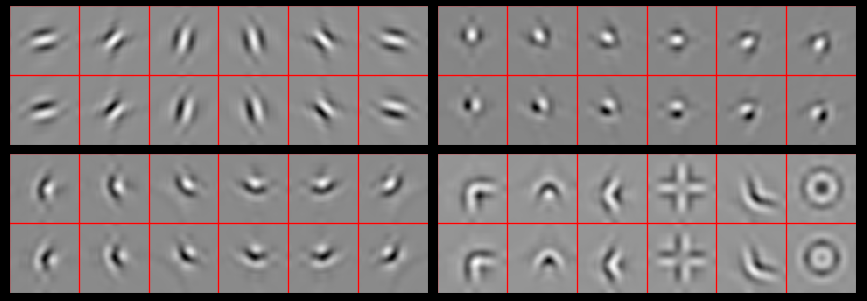
\includegraphics[width=0.9\textwidth]{\imgpath/figure3.png}
  \mycaption{Shapes possible by filtering across the wavelet orientations with
  complex coefficients}{All shapes are shown
  in pairs: the top image is reconstructed from a purely real output, and the
  bottom image from a purely imaginary output. These `real' and `imaginary' shapes
  are nearly orthogonal in the pixel space (normalized dot product $<0.01$ for
  all but the doughnut shape in the bottom right, which has $0.15$) but produce
  the same $U'$, something that would not be possible without the complex
  filters of a ScatterNet.  Top left - reconstructions from $U_1$ (i.e.\ no
  cross-orientation filtering). Top right- reconstructions from $U_1'$ using
  a $12\x 1\x 1$ Morlet Wavelet, similar to what was done in the `Roto-Translation'
  ScatterNet described in \cite{sifre_rotation_2013, oyallon_deep_2015}. Bottom
  left - reconstructions from $U_1'$ made with a more general $12\x 1\x 1$
  filter, described in \autoref{eq:ch4:simple_corner}. Bottom
  right - some reconstructions possible by filtering a general $12\x 3\x 3$ filter.}
  \label{fig:ch4:newshapes}
\end{figure}

% The work in \cite{oyallon_deep_2015} demonstrated that second order scattering
% coefficients are necessary, and give a large increase in accuracy over using
% just the first order coefficients.
% We now propose an additional layer that can be added to our
% ScatterNet with ease, which generates filters sensitive to these higher order
% shapes. In fact, we have a great deal of flexibility with what shapes we can be
% sensitive to.
As a final part of this chapter, we would like to highlight some of the filters
possible by making small modifications to the ScatterNet design. The
visualizations shown here are mostly inspirational, as we did not see any marked
improvement in using them as a fixed front end for the ScatterNet system.
However, they are the basis for the next chapter of work in adding learning in
between Scattering layers.

\citeauthor{sifre_rotation_2013} introduced the idea of a `Roto-Translation'
ScatterNet in \cite{sifre_rotation_2013}. Invariance to rotation could be made
by applying averaging (and bandpass) filters across the $K$ orientations from
the wavelet transform \emph{before} applying the complex modulus. Let us call
the averaging and bandpass filters they use $h \in \complexes[K]$.
We can think of this stage as stacking the $K$ outputs of a
complex wavelet transform on top of each other and convolving a filter
$h_\alpha$ over all spatial locations of the wavelet coefficients $W_m x$.
Let us call the output from filtering across the channel dimension $V_m$:
% (this is equivalent to how filters in a CNN are fully connected
% in depth):
\begin{equation}
  V_m x(j, \alpha, \xy) = \sum_{\theta} W_{m}x(j, \theta, \xy) h_{j, \alpha}(\theta)
\end{equation}
% \end{equation}
% We then take the modulus of these complex outputs to make a second propagated
% signal:
% \begin{equation}
  % U_{m}'x \definedas |V_{m}x| = |W_{m}x \conv h| = |U_{m-1}x
  % \conv \psi_{\lambda_{m}} \conv h|
% \end{equation}

We present a variation on this idea by filtering with a more general
$h\in \complexes[12\x H\x W]$. We use 12 channels rather than 6, as we use
the $K=6$ orientations and their complex conjugates; each wavelet is a 30$\degs$
rotation of the previous, so with 12 rotations, we can cover the full
$360\degs$.
% The filters can be shared across scales J to produce the same shapes at
% different scales. Further, if $F\in \complexes[1\x 1\x 12]$, then we can
% create 12 orientations of the same shape by simply rotating the
% filter coefficients in $F$ by one sample along the third dimension; each sample
% shift rotating the shape by $30\degs$. For more general shaped $F$, we can still
% trivially get rotations of the shape, but it requires rotating the coefficients
% spatially too.

\autoref{fig:ch4:newshapes} shows some reconstructions from these $V$ coefficients
with hand-designed $h$'s using the above DeScatterNet.
All shapes are shown in real and imaginary Hilbert-like pairs; the top row of
images in each quadrant are reconstructed from a purely real $V$, while the bottom row
are reconstructed from a purely imaginary $V$.

In the top left, we display the 6 wavelet filters for reference. In the top
right of the figure we see some
of the shapes made by using the $h$'s from the Roto-Translation ScatterNet
\cite{sifre_rotation_2013, oyallon_deep_2015}.  The bottom left is where we
present some of our novel kernels. These are simple corner-like shapes made
by filtering with ${h\in \complexes[12\x 1\x 1]}$ where $h$ is set to
% \vspace{-10pt}
\begin{equation} \label{eq:ch4:simple_corner}
  h = [1, j, j, 1, 0, 0, 0, 0, 0, 0, 0, 0]
\end{equation}
The six orientations are made by rolling the coefficients in $h$ along one
sample (i.e. $[0, 1, j, j, 1, 0,\ldots]$, $[0,0,1,j,j,1,0,\ldots]$,
$[0,0,0,1,j,j,1,0, \ldots]$ \ldots). The six conjugate orientations then make up 
the final 6 orientations ($[0,0,0,0,0,0,1,j,j,1,0,0]$, $[0,0,0,0,0,0,0,1,j,j,1,0]$,
etc.). Coefficients roll back around (like circular convolution) when they reach the end. 
The canonical filter is then $[1, j, j, 1]$ where the $90\degs$ phase offset of the 
middle two weights from the outer two allows for nicely continuous ridges of 
similar intensity around the centre of the corner.

Finally, in the bottom right we see shapes made by
${h \in \complexes[12\x 3\x 3]}$. Note that with the exception of the
ring-like shape which has 12 non-zero coefficients, all of these shapes were
reconstructed with $h$'s that have 4 to 8 non-zero coefficients of a possible
64. These shapes are now beginning to more closely resemble the more complex
shapes seen in the middle stages of CNNs.

The shapes in the bottom row of the bottom right quadrant appear very similar to
those in the top row but have nearly zero inner product. This shows one level of
invariance of this system, as after taking the complex magnitude, both the top
and the bottom shape will activate the network with the same strength. In
comparison, for the purely real filters of a CNN if the top shape would cause a
large output then the bottom shape would cause near 0 activity.

% \subsection{A review of what we have done so far}
% This was inspired by our recent work with creating 12 tap complex filters
% that worked across the 6 $\DTCWT$ orientations (and their complex conjugate).
% We found that having symmetric filters, with a $90\degs$ offset between
% taps created a nice corner like object. In fact, we could then shift these
% filters along to the next coefficients and the output would rotate by
% $30\degs$ (as we'd simply used the next set of wavelet coefficients).\\\\
% Let us give a concrete example. Consider the 4 tap filter:
% $$\left[1, j, j, 1\right]$$
% Now consider the result of doing a forward transform on a $N\x N$ sized
% image. The highpass outputs (let us call them Yh) have size $2^{-k}N \x 2^{-k}N \x 6$ for each
% scale, k.
% When we  put the above filter into the first 4 $\DTCWT$ coefficients at
% the same spatial position $(x,y)$ at given scale, $k$ i.e.\
  % \begin{lstlisting}
  % Yh[k][y,x,0] = 1
  % Yh[k][y,x,1] = j
  % Yh[k][y,x,2] = j
  % Yh[k][y,x,3] = 1
  % \end{lstlisting}
% and then do the inverse $\DTCWT$, we get the result shown in
% \autoref{fig:one_corner}. Doing this is equivalent to the deconvolution of
% Zeiler and Fergus. What we're really seeing in \autoref{fig:one_corner} is
% the input shape that would give the highest response if we applied a $\DTCWT$
% to it, and then applied the above filter across the orientations.

% \begin{figure}[!h]
  % \centering
  % 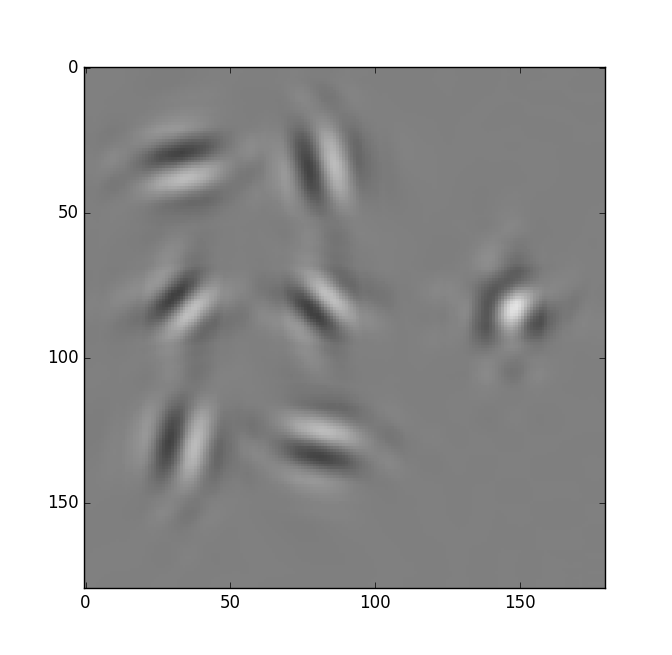
\includegraphics[scale=0.6]{\imgpath/simple_corner.png}
  % \caption{Left of image shows the imaginary part of 6 $\DTCWT$ impulse responses. Right of image
           % shows the effect of combining with the filter $\left[1, j, j, 1\right]$}
  % \label{fig:one_corner}
% \end{figure}

% If we were now to expand our definition of the above filter to be:
% \begin{equation}
  % \bmu{f} = [1, j, j, 1, 0, 0, 0, 0, 0, 0, 0, 0]
% \end{equation}
% and denote the circular shift of $f$ by k poistions to be $f_k$, then the
% output from shifting f through all 12 positions is shown in
% \autoref{fig:all_corners}. In particular, it is the first shape rotated by
% $30\degs$ for each k.

% \begin{figure}[!h]
  % \centering
  % 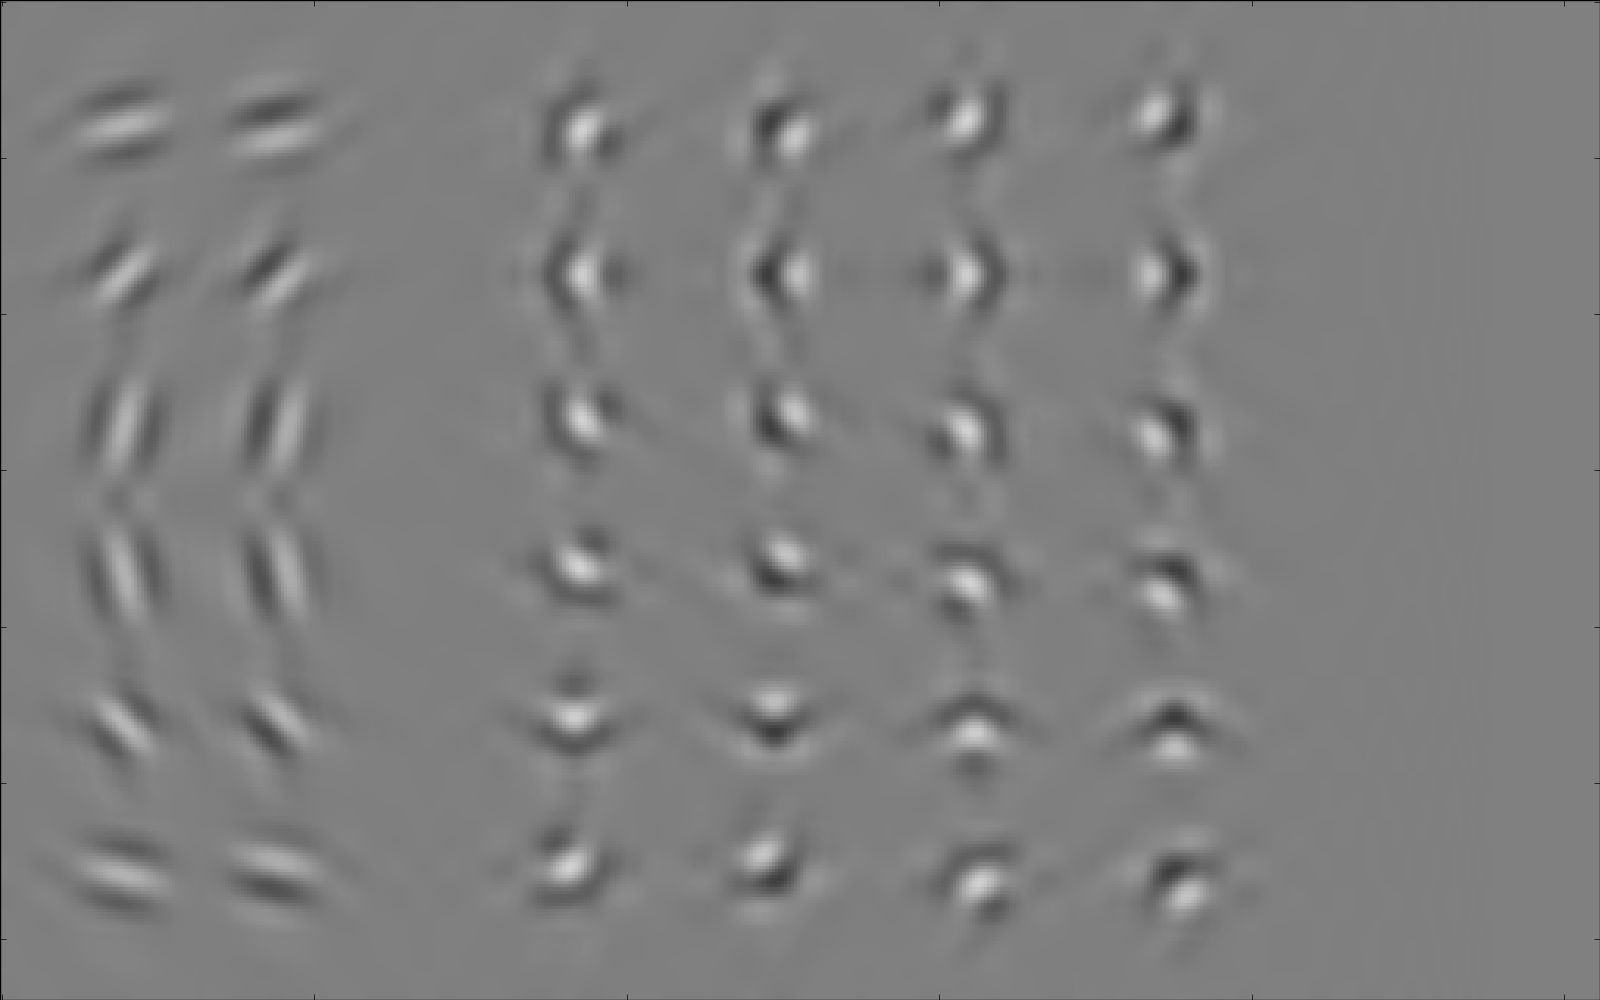
\includegraphics[scale=0.35]{\imgpath/corners_nocross.png}
  % \caption{Left shows the 6 real and imaginary $\DTCWT$ impulse responses.
  % Right of image shows the resulting 12 corners achieved from rotating
  % $\left[1, j, j, 1\right]$ through the 12 of these. The even columns are the
  % `Hilbert pair' of the odd columns, obtained by shifting all the
  % coefficients by $90\degs$ (i.e.\ $\left[j,-1,-1,j\right]$).}
  % \label{fig:all_corners}
% \end{figure}



